%A massive volume of multimodal content is generated and consumed by users around the world. 
%40\% of users report they follow content creators online where 30\% of overall 
%Many users have made a purchase following online recommendations. 
Contemporary online multimodal platforms 
%including augmented/virtual reality, 
provide an appealing rich user experience from social media to e-commerce online shopping. 
%A common characteristic of these platforms is that u
Users 
%tend to 
may promote or market their ideas, products, or personal brands through a combination of various types of modalities, such as text and images, to 
attract consumer attention.
%draw the attention of other users. 
However, the 
%nuanced 
properties of effective online multimodal marketing campaigns %present challenges for 
challenges computational analysis.
%, such as capturing contextual congruence.  
Potentially, synergy across the multi-sensory information space facilitates faster and more accurate processing to establish semantic relationships \cite{laurienti2004semantic,spence2011crossmodal,wickens2008multiple}. However, 
%rich, user-generated 
%multimodal content challenges 
the computational modeling of multi-modal content 
%often relies on the detection of implicit patterns in large corpora that 
makes little explicit contact with human knowledge, experience, and reasoning.
%in lieu of explicit analysis that aligns with readily accessible human interpretation. 
%human-accessible semantics. 
The smaller, earlier (multimodal) Visual Language Models (VLMs) such as MMBT \cite{kiela2020supervised}, ViLBERT \cite{lu2019vilbert} and LXMERT \cite{tan2019lxmert} 
%were limited in identifying congruent contextual cues
%, despite their intuitive designs. 
%These VLMs often 
typically exploit independent unimodal cues (e.g., textual, visual) connecting the image and text.
%, which do not capture the explicit multimodal semantic relationships. 
More recent very large VLMs, such as LLaVA \cite{liu2023visual}, BLIP2 \cite{li2023blip} and GPT-4 \cite{openai2023gpt4}, do capture  \emph{implicit} multimodal semantic relationships,  but without semantic constraints, making them vulnerable to 
%to the extent that they suffer from 
hallucinations--- \emph{superficially congruent} \cite{hasanyou,Meyer2022-cf} and  \emph{catastrophically incorrect} \cite{shuster2021retrieval,Maynez2020-cj}. Moreover, these models often remain unable to identify the explicit semantic connections between modalities that influence human interpretation. \cite{ji2020leveraging}. 
%Hence, utilizing these unconstrained models off-the-shelf without taking helpful measures such as grounding and contextualizing, 
Such models are simply %not up to the task of 
unable to  assess computationally compelling multimodal online marketing campaigns 
%independent of their are misleading and in some cases may pose real risks when used on sensitive topics, such as 
%elections, social issues 
\cite{mcguffie2020radicalization,weidinger2022taxonomy,tamkin2021understanding,de2023chatgpt}. 

Consider the image and text in Figure \ref{fig:image-womens-movement-patriachy}, drawn from our dataset. 
%One can see in the image 
The image contains two women smiling with the saga sign along with the text \emph{"Let's Go!"}. The intended holistic meaning can be determined only after seeing the actual caption \emph{"Smash the glass ceiling. Destroy the patriarchy. Save the record store."} The creator of this marketing campaign seemingly intended to promote women's representation in society and the music industry by using an image of two assertive and confident women in the image. The pictured women are in fact the unstated subjects of smashing, and as such, destroying male dominance enshrined in patriarchy. Hence, to capture the correct meaning of a pair of images and text, it is crucial to see both modalities and form contextually informed connections.
%between them. 

% \vspace{-0.2em}
\begin{figure}[hbt!]
  \centering
  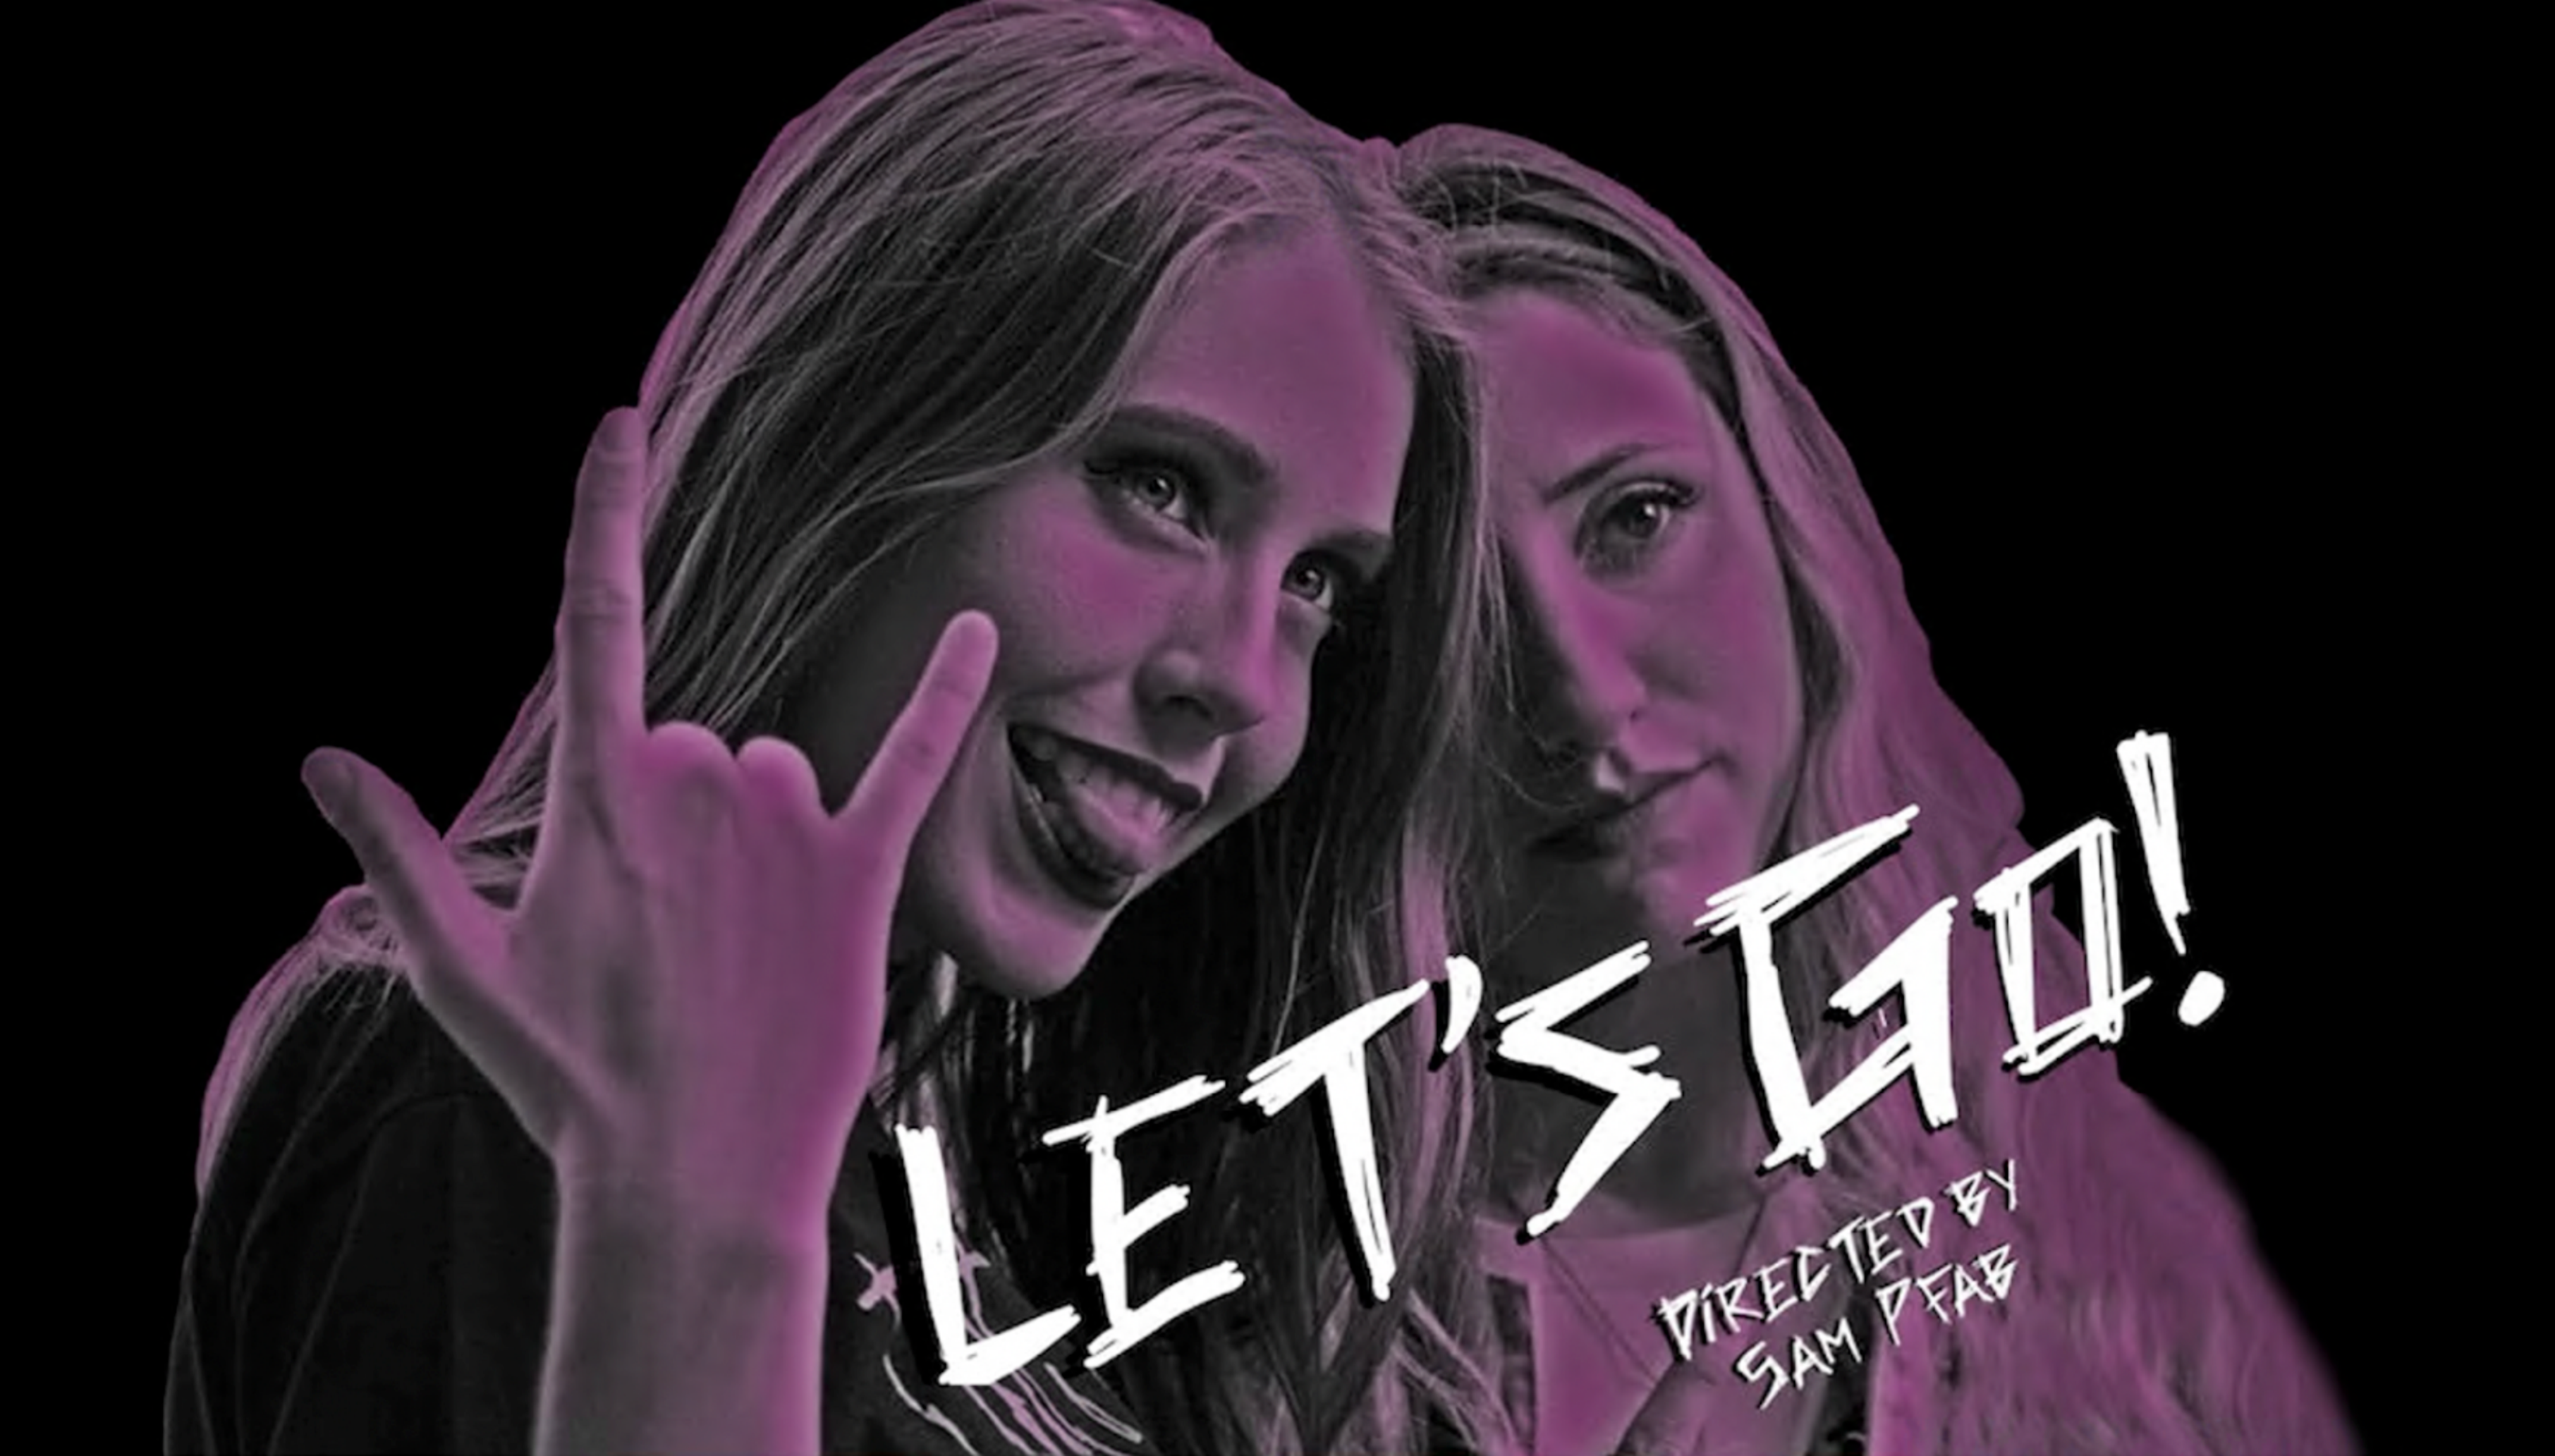
\includegraphics[width=8.5cm]{Figures/record_store_protest-2.pdf}
\vspace{-1.3em}
\caption{An example pair of image and human caption text from our crowdfunding dataset. The caption generated by the BLIP model and the actual human-generated caption of the image is below. 
\textbf{BLIP caption:} "Two women smiling with a hand gesture of rock and roll." 
\textbf{Actual human caption:} "Smash the glass ceiling. Destroy the patriarchy. Save the record store."}
\vspace{-1em}
\label{fig:image-womens-movement-patriachy}
\end{figure} 

Table \ref{tab:generated-caption-two-women} provides the generated explanations using SOTA multimodal models including BLIP2, and LLava. 
%Overall, 
While LLava \cite{liu2023visual} did generate explanations of the input pair with a  contextually informed meaning, it suffers from hallucinations, such as “The image features two women standing next to each other, \emph{both holding their cell phones in their hands. They seem to be taking selfies}”. In the given image, there are no cell phones nor are they taking selfies.
%is no sign of women holding their cell phones.
%, while the model claims otherwise. 
For comparison, we queried ConceptNet {\cite{speer2018conceptnet}} to extract the most relevant concepts, and simply appended these to the pair of text and image as input to these models. As expected, the generated output does mitigate hallucinations (see Table \ref{tab:generated-captions} in Appendix). This %point is 
shows that multimodal analysis guided by external knowledge %improves performance by making 
makes more reliable inferences by forming cross-modal contextual connections. 

%Researchers have studied the hallucination problem in several use cases including text summarization \cite{huang2021factual} and dialogue generation \cite{shuster2021retrieval}, showing how retrieval-augmented multimodal models can generate enhanced and grounded representations with external knowledge. 

%One problem with existing methods is a lack of congruence between the interpretation of the image and the associated text. 
%Our emphasis on multimodal congruence introduces a measurement problem. 
We introduce here the notion of \emph{multimodal congruence.} We measure multimodal congruence 
%learned by multimodal models 
%through measuring the 
using the semantic distance between the separate image and caption (text) representations, 
as this distance is 
expected to be shorter in a congruent multimodal representation \cite{mandera2017explaining,frank2017word,beck2011congruence,maki2004semantic}. We can then demonstrate how external knowledge can enhance and contextualize the representations to close the semantic gap between the modalities. In doing so, we can better predict the success of marketing campaigns.  
% TK: Interesting discussion - if you can later present how to generate an embedding of the semantics of image and caption and formally measure their distance and then motivate how to bridge it with what consequence, it will be neat!

%Our approach incorporates external knowledge in a multimodal learning framework. 
In this study, we answer the following two research questions: \\
\textbf{RQ1:} Can we 
%explore and 
improve the contextual congruence of the representations of multimodal content by incorporating external knowledge while learning to unveil subtle cross-modal semantic relationships? \\
\textbf{RQ2:} Do more contextually congruent representations help the model obtain more consistent and reliable predictive performance for the success of multimodal marketing campaigns? %effectiveness? 

Our technical approach incorporates  an external commonsense Knowledge Graph (KG) (e.g., ConceptNet) 
%incorporated 
to learn knowledge-infused multimodal representations of the data. We first take pairs of images and text from our dataset and generate embeddings using text and image encoders (i.e., via LLMs, LVMs). To query the KG, %ConceptNet, 
we generate captions for images using BLIP \cite{li2022blip}. Then, we retrieve the most similar concepts from ConceptNet based on semantic search. We train knowledge graph embedding (KGE) models to generate representations of the resulting concepts. Initially, we learn multimodal data representations using bidirectional transformers. These representations are then fused with the KGEs through a linear and a multi-head cross-attention layer. 

The novelty of our work lies in modeling a social and behavioral problem, such as effective marketing, utilizing neural and symbolic models \cite{sap2022neural}. In so doing, we particularly addressed the problem of learning a contextually enhanced neural representation of multimodal content with external commonsense KG (i.e., symbolic) \cite{yu2022probabilistic,kursuncu2020kil}. This helps the model to better capture the holistic meaning across modalities enhancing model performance in predicting the success of multimodal marketing campaigns.
% %Our experiments involving 
% Utilizing multiple LLMs and LVMs coupled with KGEs, we demonstrate the 
% %difference in 
% performance advantage for predicting the success of multimodal marketing campaigns.  
%We observe that the 
%Representations enhanced with explicit contextual information help models form semantic connections between modalities. 
Knowledge-infused multimodal models outperform other models without knowledge. Error analysis (see Section Results \& Discussion) reveals how external knowledge improves the capture of intended holistic multi-modal meaning. 
%Thus, we simultaneously 
We demonstrate the contribution of knowledge to machine learning algorithms 
%and to enable 
for computational analysis of marketing campaigns, which provide an ecologically valid measure of success.
%To clarify the contribution of knowledge, we provide a discussion on error analysis in our experiments as to how external knowledge improves the capturing of the intended meaning.
%This contextualization proves to be impactful in a downstream task in marketing. 
%While t
%The findings indicate the critical contribution of external knowledge from a KG to the machine understanding of multimodal content.
%, there is much to explore in incorporating knowledge for contextualizing multimodal representations.

\begin{table*}[hbt!]
\vspace{-0.2em}
  \centerline{
    \begin{tabular}{p{0.8cm}p{1.3cm}p{14.2cm}}
    \toprule[2pt]
   \textbf{\centering Model} & \textbf{\centering Knowledge} & \textbf{Text Caption} \\
    \toprule[1pt]
    BLIP2 & \centering No & the cover of let's go with two girls posing in front of a purple background going for a protest. \\
    \toprule[1pt]
    BLIP2 & \centering Yes & The cover of a movie "let's go" which talks about patriachy in the record store. \\ 
    \toprule[1pt]
    Llava & \centering No & The image features two women standing next to each other, both holding their cell phones in their hands. They seem to be taking selfies or sharing a moment together. One of the women is making a funny face, adding a playful vibe to the picture. The other woman is simply enjoying the moment and being part of the fun. \\ 
    \toprule[1pt]
    Llava & \centering Yes & The image features two beautiful and majestic black women standing together, united in their quest to smash the glass ceiling and destroy the patriarchy. They are surrounded by record albums, highlighting their shared passion for music and the record store. Their powerful presence and determination to save the record store from any threat make for a compelling scene that showcases their strength and resilience in the face of oppressive societal norms. \\
    \bottomrule[2pt]
    \end{tabular}%
  }
\vspace{-0.5em}
\caption{For the image and text pair (see Figure \ref{fig:image-womens-movement-patriachy}), the captions generated by the models BLIP2 and Llava, when the model was prompted with the Image and Text with and without external Knowledge. The knowledge is extracted from ConceptNet as explained in section \ref{sec:explicit-knowledge} and appended to the prompt input to these models. 
%While t
\emph{The captions with generated knowledge show less hallucination.}
% and more grounding, we leave further investigation of those to the reader as they are not the focus of this study. 
For more examples, see Table \ref{tab:generated-captions} in the Appendix.}
\label{tab:generated-caption-two-women}
% \vspace{-0.2em}
\end{table*}